\documentclass[UTF8]{ctexart}
\usepackage{graphicx}
\usepackage{amsmath}
\usepackage{cite}
\usepackage{mathtools}
\usepackage[a4paper,left=2.5cm,right=2.5cm,top=3cm,bottom=3cm]{geometry}
\title{密立根油滴实验:实验报告}
\author{禤科材 PB20030874 20级14系 707组 1号台}
\date{\today}
\bibliographystyle{plain}

\begin{document}
    \maketitle

    \section{实验目的}
    \begin{center}
        通过测定电场中油滴带电量测定单位元电荷
    \end{center}
    \section{实验原理}
    在密立根油滴实验中,测量电子电荷的基本设计思想是,使带电油滴在测量范围内处于受力平衡状态。按油滴作匀速或静止两种运动状态分类,可分为动态测量法和平衡测量法。本实验使用平衡测量法测元电荷。
    
    平衡测量法的出发点是,使油滴在均匀电场中静止在某一位置,或在重力场中作匀速运动。
    当油滴在电场中平衡时,油滴在两极板间受到电场力$qE$、重力$m_1g$和浮力$m_2g$达到平衡,从而静止某一位置。即:
    \begin{equation}
        qE=(m_1-m_2)g
    \end{equation}

    重力场中一个小的油滴,半径为r,质量为$m_1$。空气是粘滞性流体,故此运动的油滴,除受重力和浮力外,还受粘滞阻力的作用。由斯托克斯定律,粘滞阻力与物体运动速度成正比。设油滴以均匀速度$v_f$下落,则有:
    \begin{equation}
        m_1g-m_2g=Kv_f
    \end{equation}
    
    此处$m_2$为与油滴同体积的空气的质量,$k$为比例系数,$g$为重力加速度。油滴在空气及重力场中
    的受力情况如下图所示:
    \begin{figure}[ht]
        \centering 
        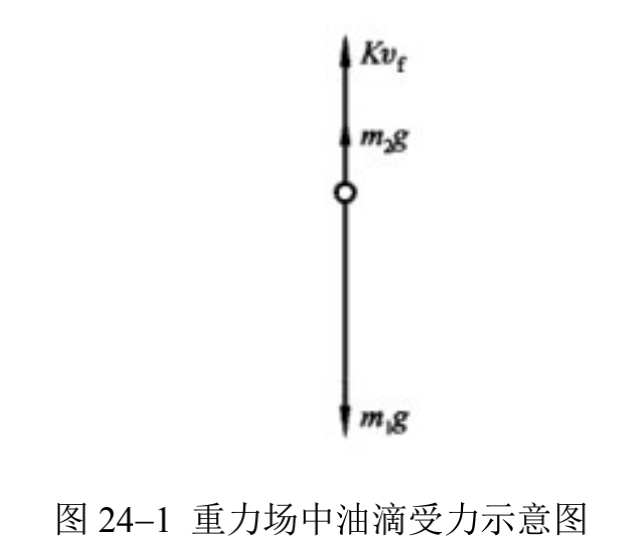
\includegraphics[width=5cm]{Screenshot 2021-05-18 at 21.37.35.png}
    \end{figure}

    由于油滴的直径已经与空气分子的间隔相当,空气已不能看成连续介质,需要对斯托克斯公式做适当修正:
    \begin{equation}
        \eta'=\frac{\eta}{1+\frac{b}{pr}}
    \end{equation}
    其中p为空气压强,b为修正常数

    油滴带电量的最终表达式为:
    \begin{equation}
        q=9\sqrt{2}\pi d[\frac{(\eta v_f)^{3}}{(\rho _1-\rho _2)g}]^{\frac{1}{2}}\frac{1}{U}[\frac{1}{1+\frac{b}{pr}}]^{\frac32}(\frac{1}{t_f})^{\frac32}
    \end{equation}
    
    将所有已知数值带入后,最终带电油滴所带电荷量为:
    \begin{equation}
        q=\frac{1.429*10^{-14}}{U_{平衡}[t_f(1+0.0196\sqrt{t_f})]^{\frac{3}{2}}}
    \end{equation}
    \section{实验步骤}
    将电压调到大于150V,向实验仪器中喷入油滴,油滴通过仪器的放电而带上不同量的电荷

    迅速调整显微镜焦距,寻找颗粒适中、速度较小、受力大约平衡的油滴

    调整电压,使得找到的油滴处于静止状态,记录此时的平衡电压

    控制电压,将油滴移动至显示屏最上方刻度线
    
    去掉外加电压并开始计时,让油滴自由下落至屏幕最下方刻度线,停止计时,记录下$t_f$

    再次提升油滴,略微调整电压,如果油滴仍然处于静止状态,则重复上述步骤

    对一个油滴测量7至8次,对其他三个油滴测量3次

    \section{实验记录}

    \begin{figure}[ht]
        \centering 
        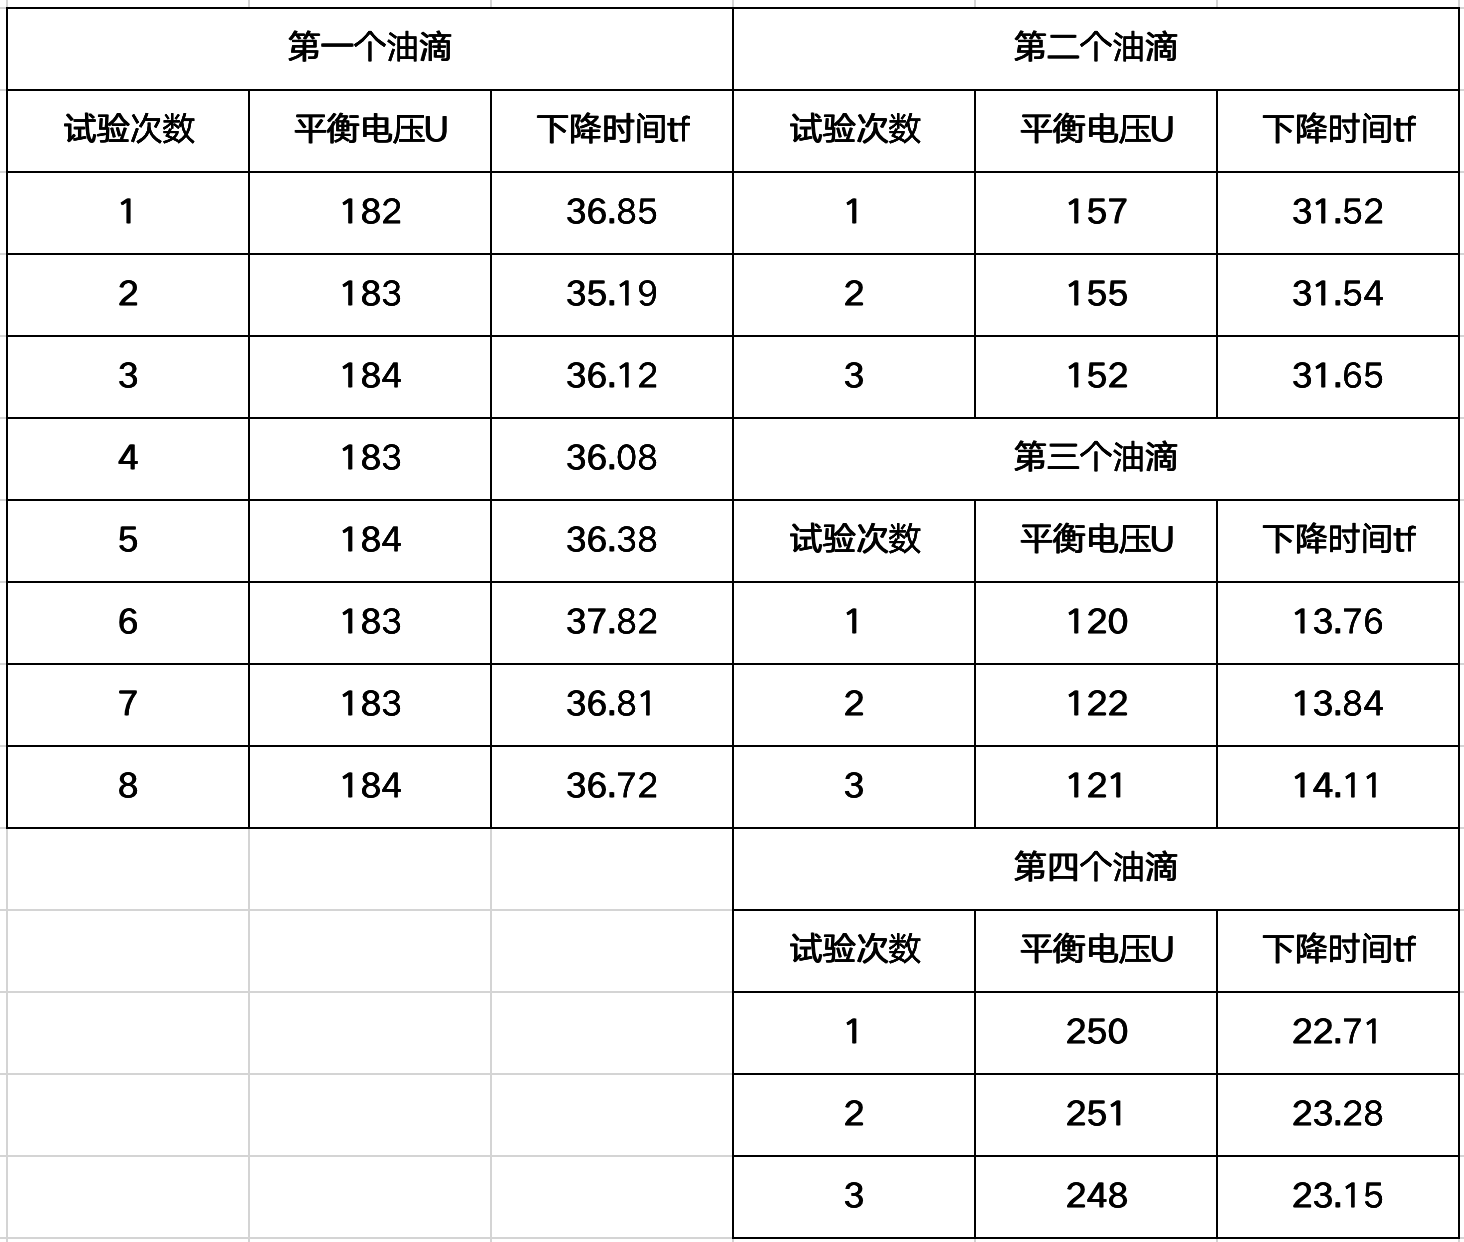
\includegraphics[width=12cm]{q.png}
    \end{figure}

    \section{数据处理}
    \begin{center}
        \emph{\zihao{4}大数据分析}
    \end{center}

    根据老师提供的大数据表,以$U$为纵轴、$w=t$为横轴,作原始散点图如下:
    \begin{figure}[ht]
        \centering 
        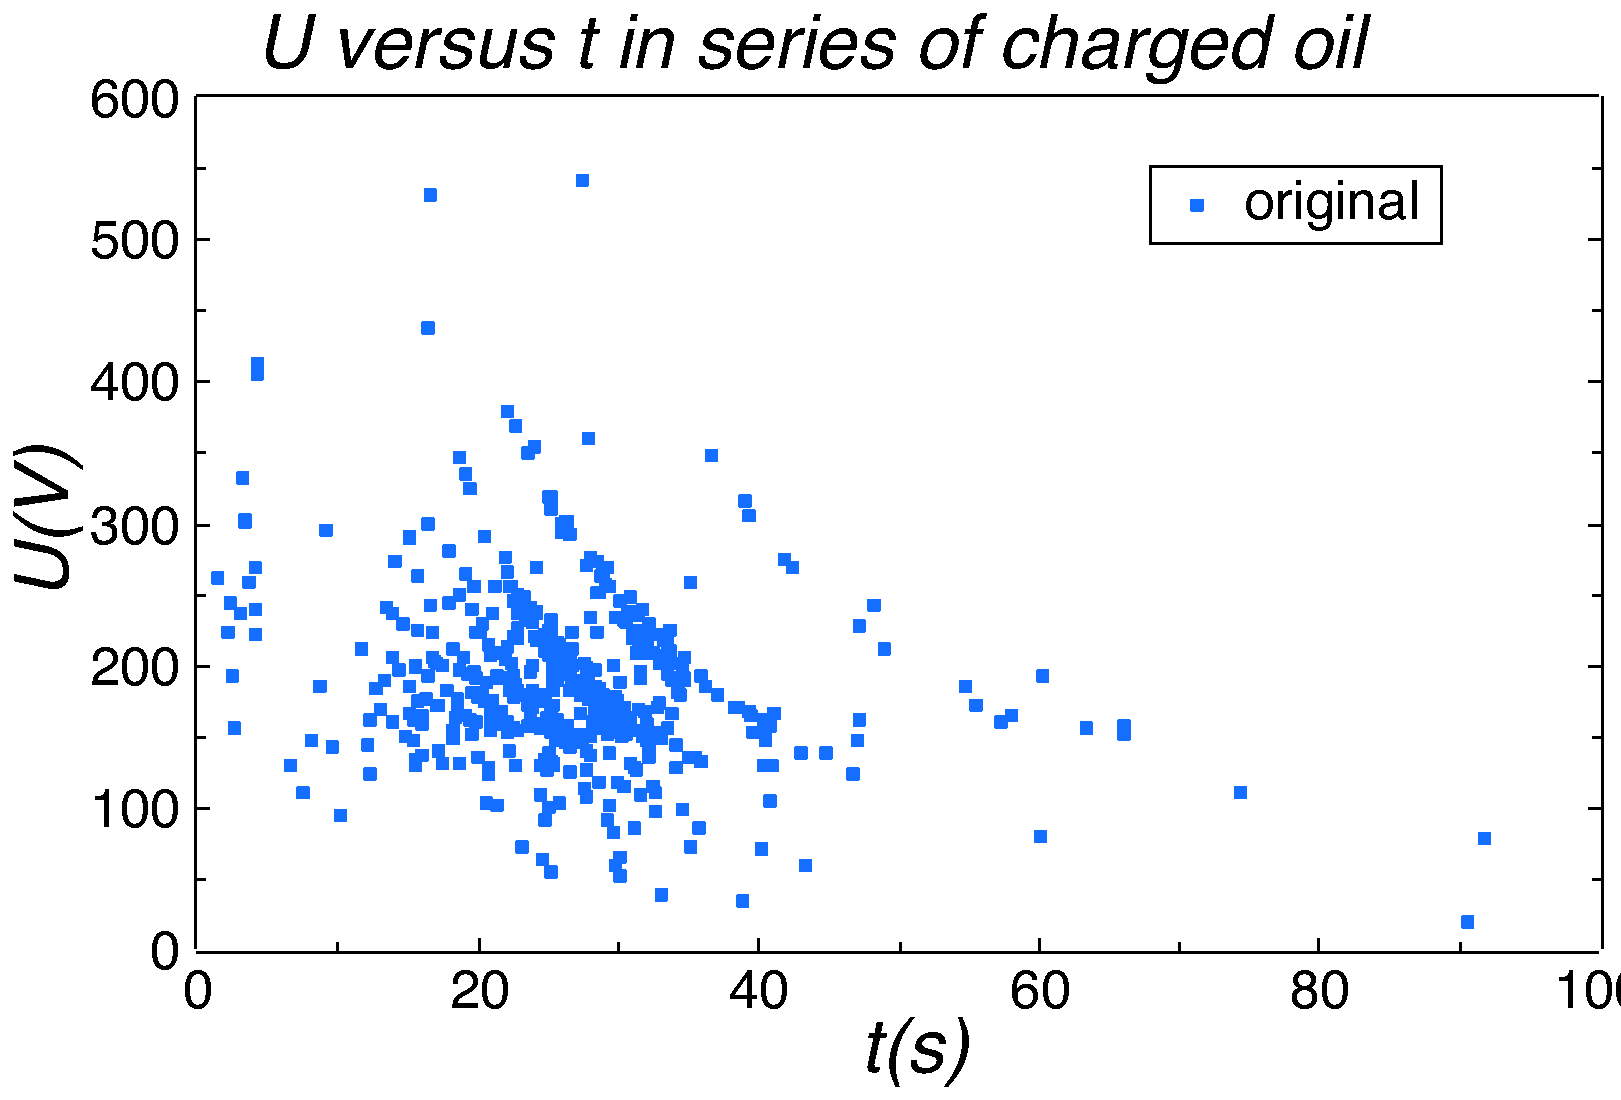
\includegraphics[width=8cm]{original.pdf}
    \end{figure}

    观察到数据点较为明显地分布在三条曲线周围,令$w=[t(1+0.0196t^{0.5})]^{1.5}$

    
    取附近的数据点重新以$\frac1U$为纵轴、$w$为横轴作图,斜率即是$\frac{q}{1.429*10^{-14}}$:
    \begin{figure}[ht]
        \centering 
        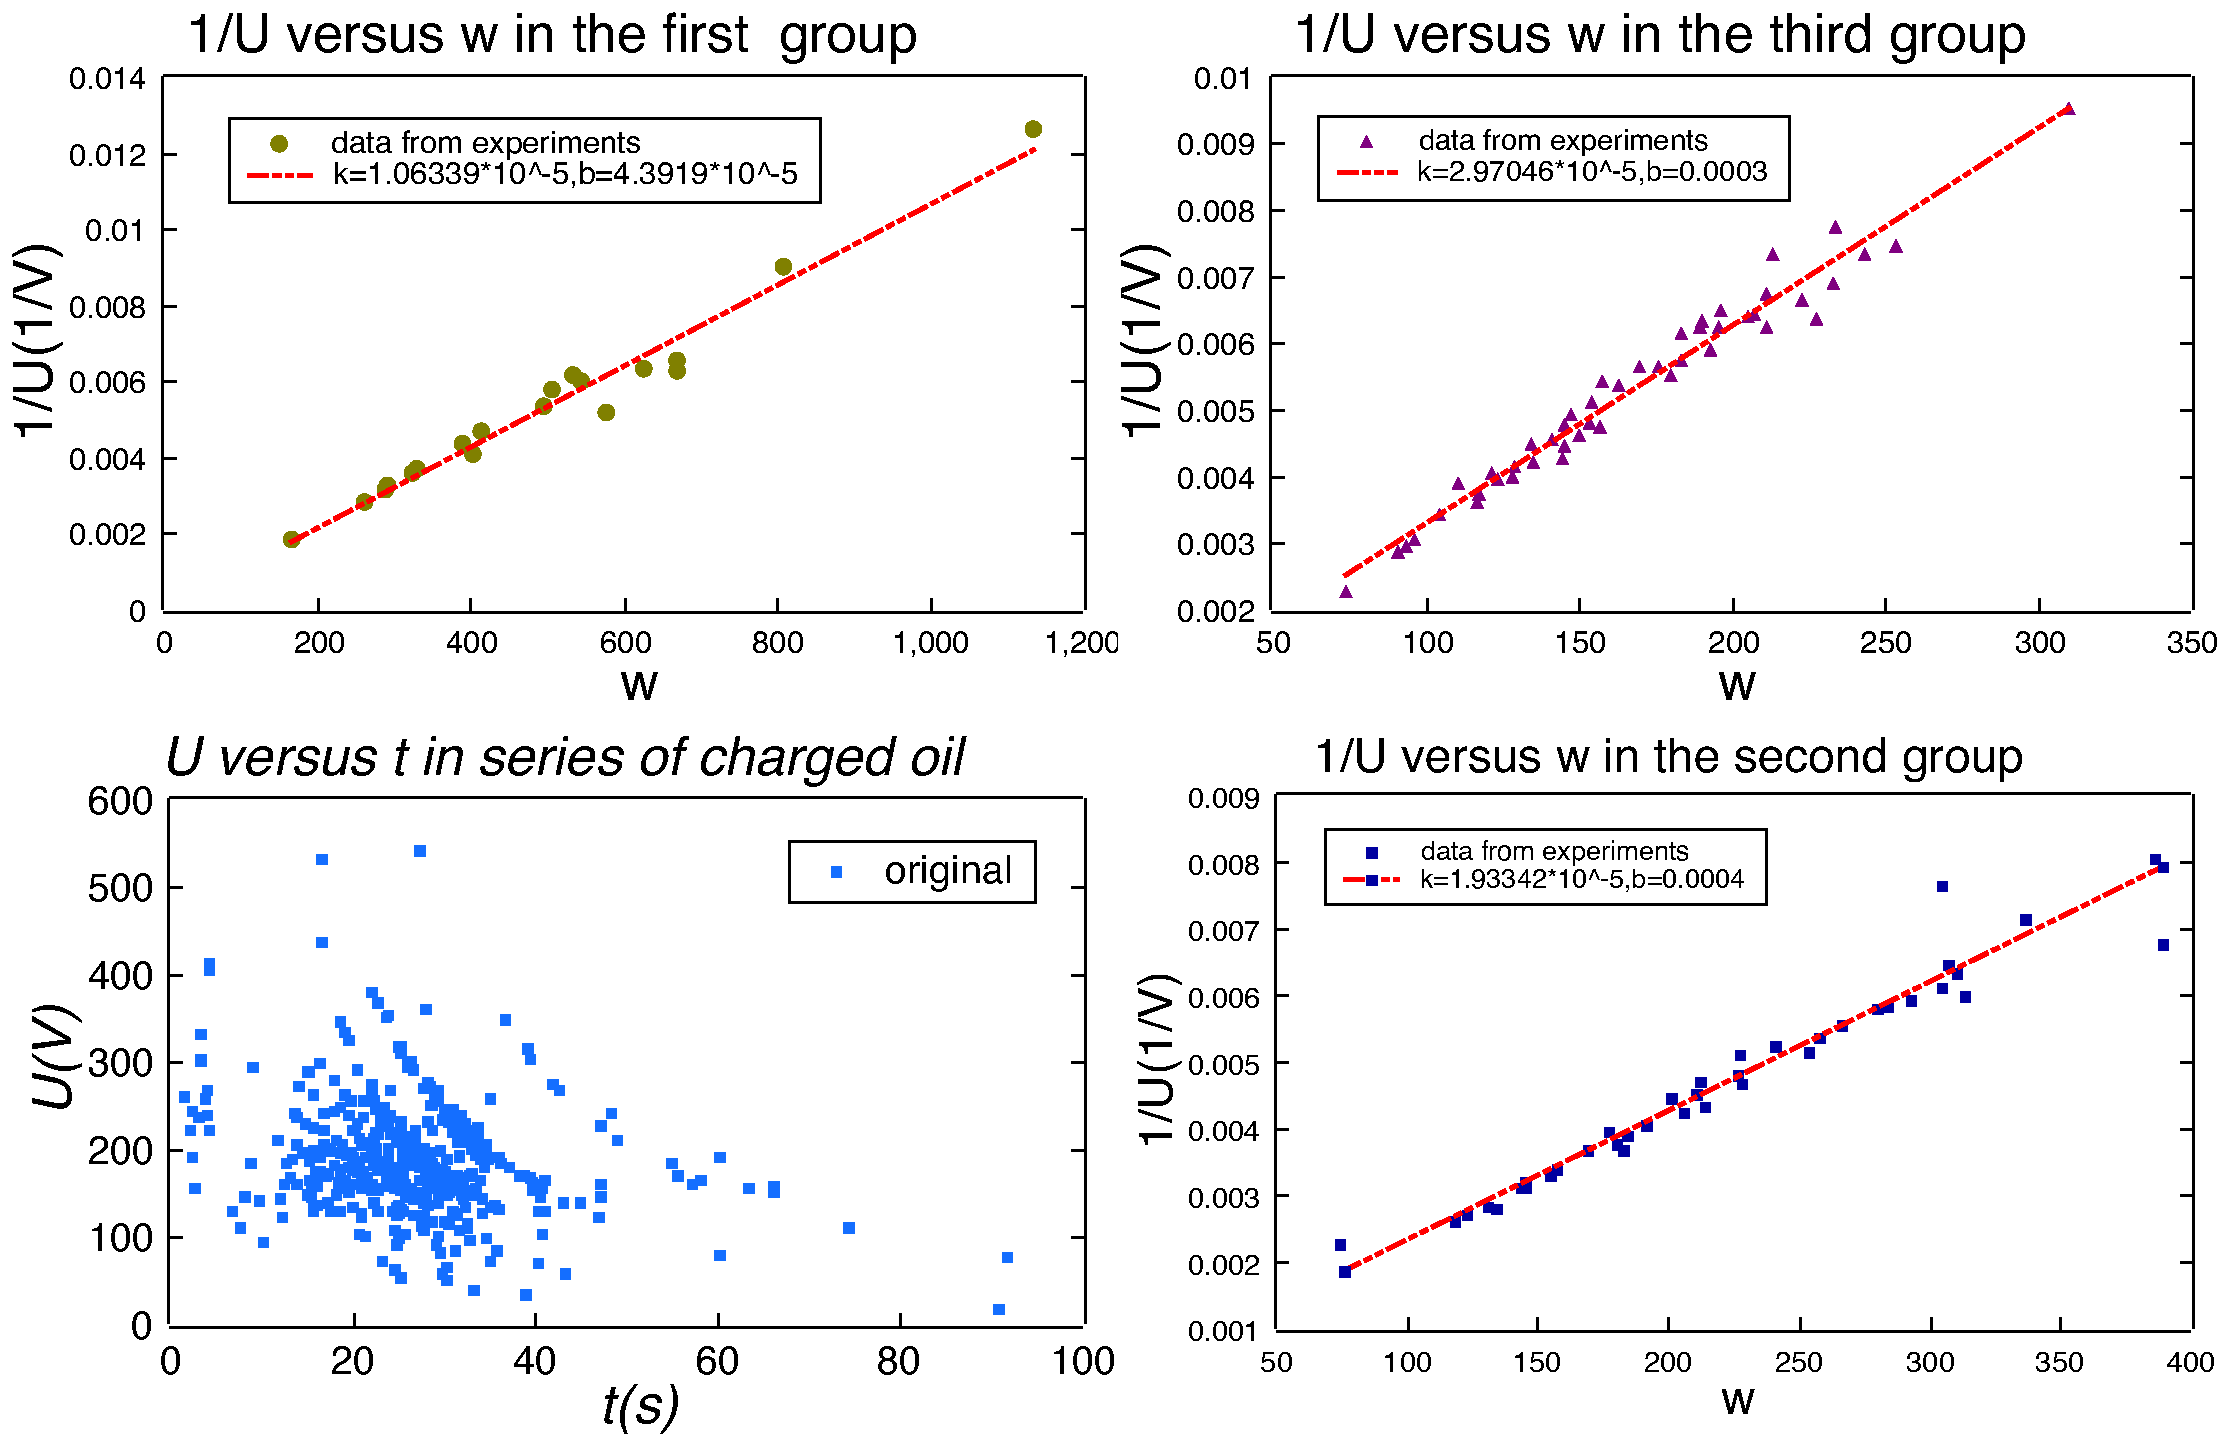
\includegraphics[width=14cm]{fimad.pdf}
    \end{figure}

    实验数据点基本分布在拟合直线两侧,表明线性相关性良好,数据可信度高。根据公式$q=k*1.429*10^{-14}$计算得到:
    $q_1=1.519*10^{-19}C$,$q_2=4.2447*10^{-19}C$,$q_3=2.7628*10^{-19}C$,分别带元电荷数目为1、3、2个
    \begin{center}
        \emph{\zihao{4}本次数据}
    \end{center}

    \emph{电压$V$平均值:}
        \begin{equation*}
            \overline{U}=\frac{182	 +183+	184+	183+	184+	184	+183	+183}{8} =183.25(V)
        \end{equation*}

        \emph{电压$V$标准差:}
        \begin{equation*}
            \sigma _{U}=\sqrt{\frac{\sum_{i=1}^8(V_i-\overline{V})^2}{8-1}} =\sqrt{\frac{3.5}{7}}=0.707107(V)
        \end{equation*}

        \emph{电压$A$类不确定度:}
        \begin{equation*}
            U_A=t_{0.95}\frac{\sigma_l}{\sqrt{n}}=2.36·\frac{0.707107}{\sqrt{8}}=0.5900(V)
        \end{equation*}

        \emph{电压$B$类不确定度:}
        \begin{equation*}
            U_{B}=k_p·\frac{\varDelta B_仪}{C}=1.96·\frac{0.5}{3}=0.326667(V)
        \end{equation*}

        \emph{电压$U$展伸不确定度(P=0.95):}
        \begin{equation*}
           U_{V}=\sqrt{UA^2+U_B^2}= \sqrt{0.5900^2+0.326667^2}=0.674397(V)
        \end{equation*}


        \emph{时间$t$平均值:}
        \begin{equation*}
            \overline{t}=\frac{36.85	+35.19+	36.12	+36.08+	36.38	+37.82+	36.81	+36.72}{8} =36.49625(s)
        \end{equation*}

        \emph{时间$t$标准差:}
        \begin{equation*}
            \sigma _{U}=\sqrt{\frac{\sum_{i=1}^8(t_i-\overline{t})^2}{8-1}} =\sqrt{\frac{4.0605875}{7}}=0.761632(s)
        \end{equation*}

        \emph{时间$A$类不确定度:}
        \begin{equation*}
            U_A=t_{0.95}\frac{\sigma_l}{\sqrt{n}}=2.36·\frac{0.761632}{\sqrt{8}}=0.635495(s)
        \end{equation*}

        \emph{时间$B$类不确定度:}
        \begin{equation*}
            U_{B}=k_p·\frac{\varDelta B_人}{C}=1.96·\frac{0.2}{3}=0.130667(s)
        \end{equation*}

        \emph{时间$t$展伸不确定度(P=0.95):}
        \begin{equation*}
           U_{t}=\sqrt{UA^2+U_B^2}= \sqrt{0.635495^2+0.130667^2}=0.648790(s)
        \end{equation*}

        \emph{\zihao{4}结果:}
        \begin{equation*}
            q=\frac{1.429*10^{-14}}{183.25[36.49625*(1+0.0196\sqrt{36.49625})]^{\frac{3}{2}}} =2.9903*10^{-19}(C)
        \end{equation*}

        \emph{根据不确定度合成公式:}
        \begin{equation}
            \frac{U_q}{U}=\sqrt{(\frac{U_V}{U})^2+(\frac32 *\frac{U_t}{t})^2+(\frac32 * \frac{0.0196U_t}{(1+0.0196\sqrt{t})*2\sqrt{t}})^2}
        \end{equation}

        \begin{equation*}
            \frac{U_q}{U}=\sqrt{(\frac{0.674397}{183.25})^2+(\frac32 *\frac{0.648790}{36.49625})^2+(\frac32 * \frac{0.0196*0.648790}{(1+0.0196\sqrt{36.49625})*2\sqrt{36.49625}})^2}=0.026955
        \end{equation*} 

        \emph{\zihao{4}最终结果:}
        \begin{equation*}
            q_1=2.99(1±0.027)*10^{-19}(C)
        \end{equation*} 
        \begin{equation*}
            q_2=4.45*10^{-19}(C)
        \end{equation*}
        \begin{equation*}
            q_3=2.05*10^{-18}(C)
        \end{equation*}
        \begin{equation*}
            q_4=4.52*10^{-19}(C)
        \end{equation*}

        \emph{故带元电荷数量分别为:}
        \begin{equation*}
            n_1=2
        \end{equation*}
        \begin{equation*}
            n_2=3
        \end{equation*}
        \begin{equation*}
            n_3=10
        \end{equation*}
        \begin{equation*}
            n_4=3
        \end{equation*}
        本次实验误差较大:控制秒表0.2s的误差;由于微小油滴的布朗运动,一些油滴在确定平衡电压时是否静止判断不准确,导致测得的平衡电压其实并不是真实的平衡电压;还有仪器本身存在误差及当时实验的环境影响,所以本试验有较大误差。但在教学实验要求范围内,可以认为本实验结果符合要求

        \emph{以所带元电荷数目为X轴,带电量为Y轴,作图,则斜率即是元电荷电量:}
        \begin{figure}[ht]
            \centering 
            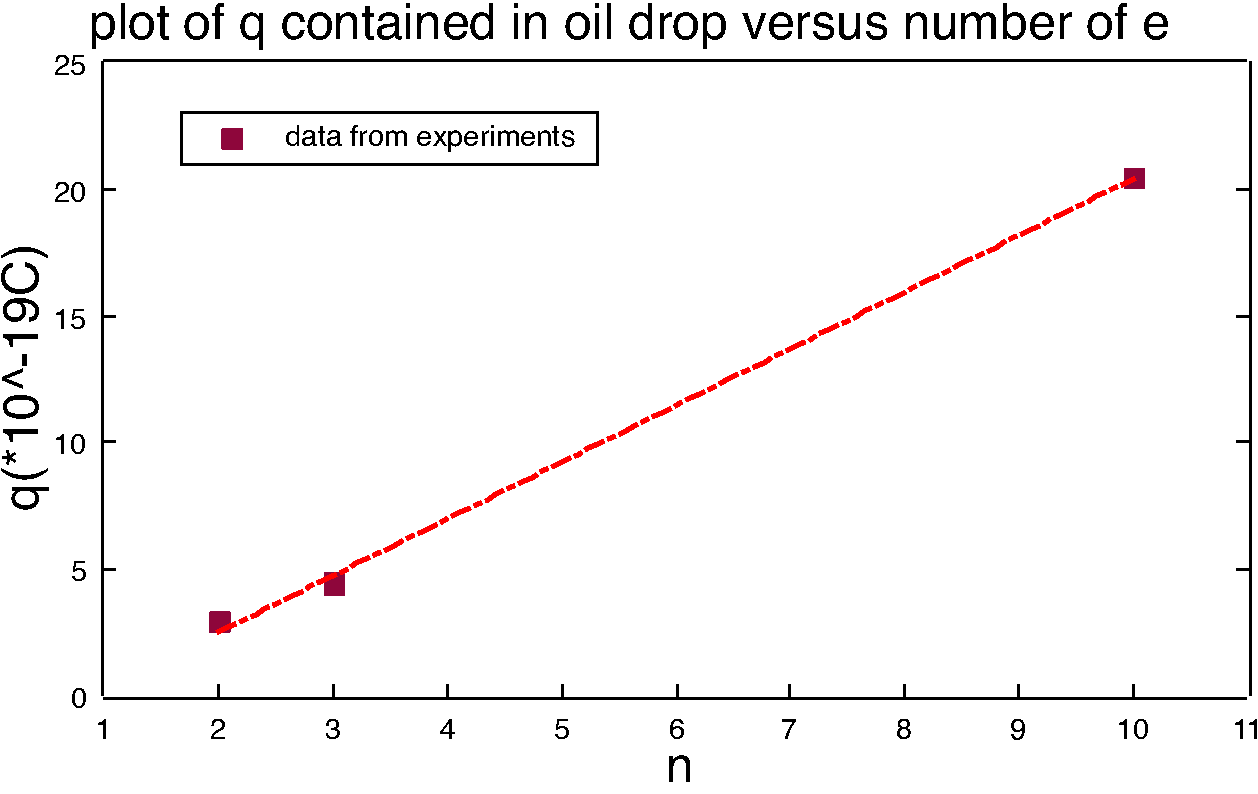
\includegraphics[width=8.5cm]{www.pdf}
        \end{figure} 

        \emph{\zihao{4}线性拟合后结果为$e=2.239*10^{-19}(C)$}

    \section{数据汇总}
    \begin{figure}[ht]
        \centering 
        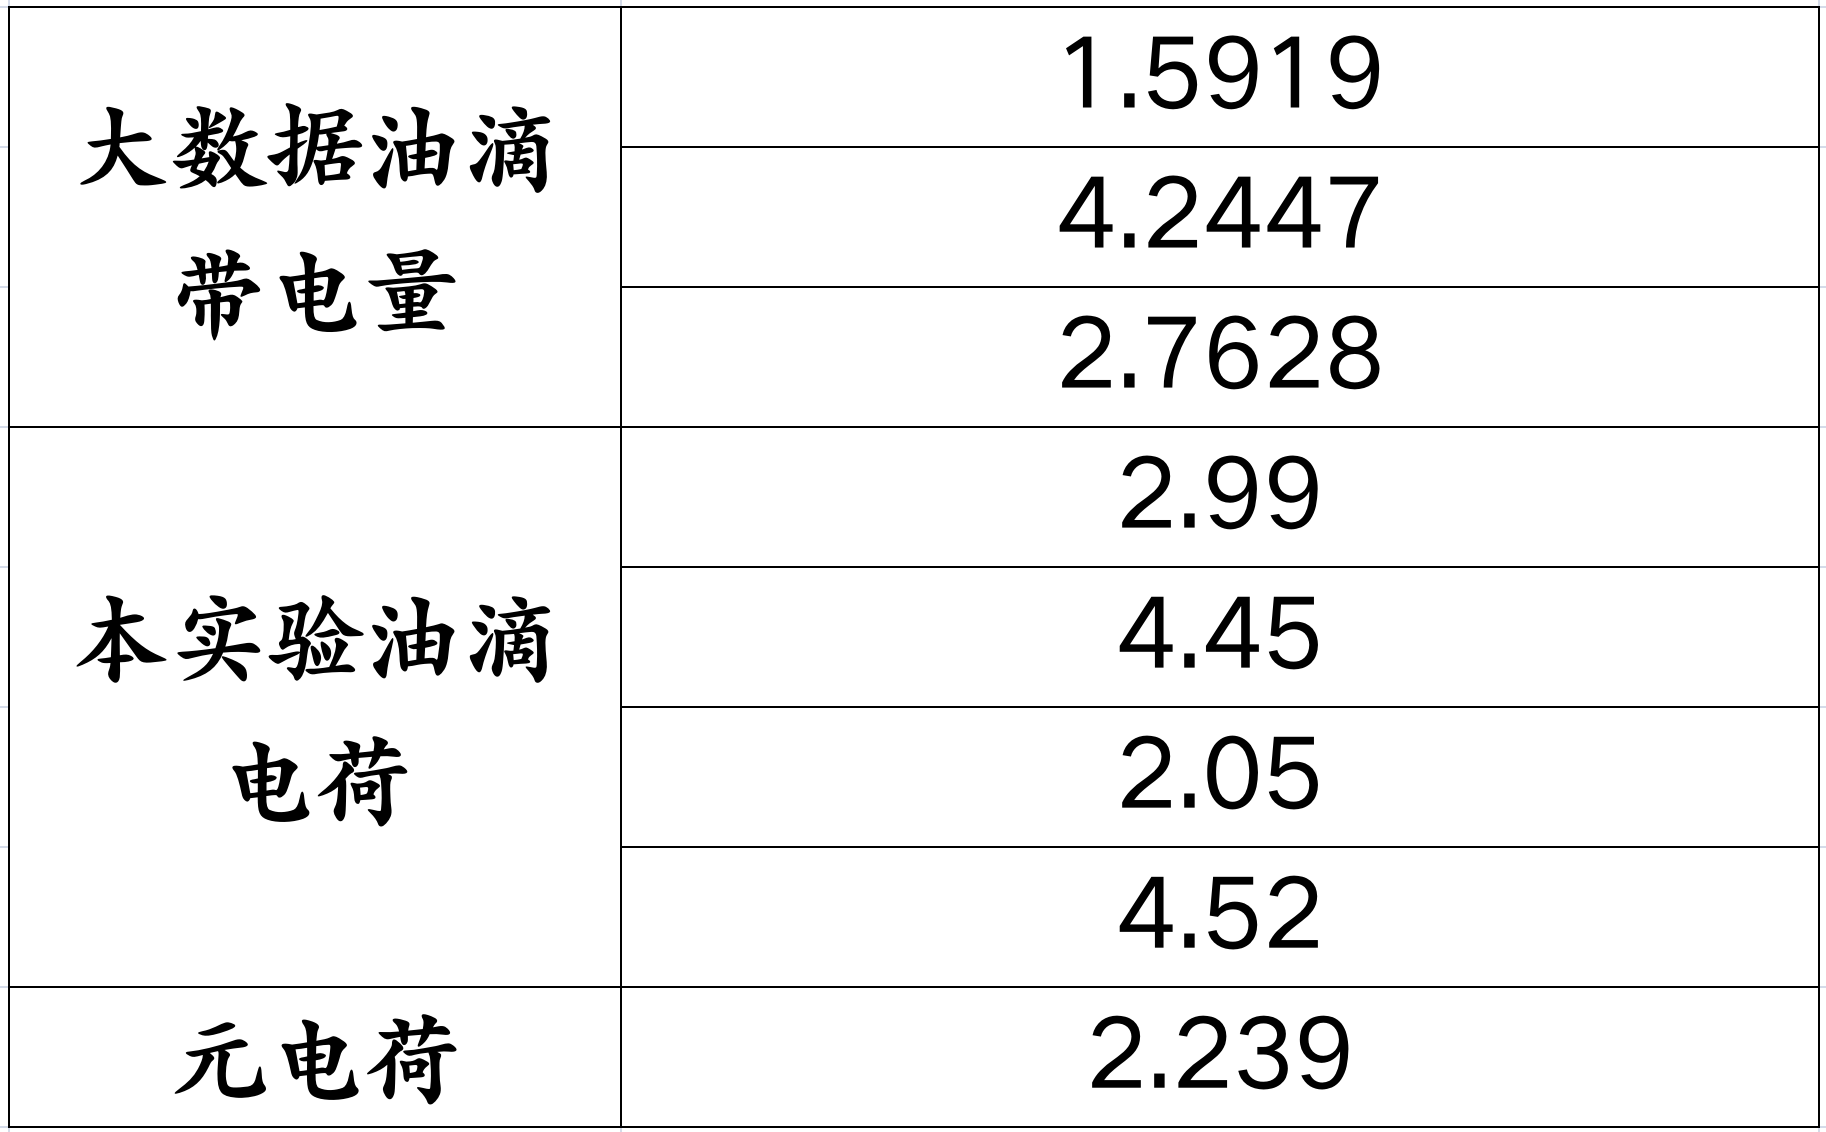
\includegraphics[width=7cm]{ddd.png}
    \end{figure} 
    \section{误差分析}
    元电荷公认值为$1.602*10^{19}$库仑,大数据分析后三组数据结果均偏小、本次实验使用线性拟合法测得的元电荷电量为$2.239*10^{-19}$库仑,数据偏大,分析可能有以下几点原因:

    \emph{对于大数据分析:}
    
    三组结果均偏小,很有可能是我选择数据时有一定的主观因素,较多偏小的数据点被选进来,以致总体偏小

    \emph{对于本次实验所做出的4个油滴数据:}
    
    第一,数据点太少,线性拟合的斜率容易受极端数据影响,不具有一定的说服力。比如如果去掉带电量$20.5*10^{-19}C$的数据点,剩下三个数据拟合直线的斜率为$1.495*10^{-19}C$,和国际公认值相比又偏小

    第二,实验时急于获得结果,没有很耐心地操作实验。实验中我其实测了8个油滴,但是大部分都不满足电压大于150V、下落时间大于15s的条件,所以必须重新调试仪器,找到符合标准的油滴。这其中消耗了大量的时间,以至于实验到很晚才结束,而且当天晚上状态欠佳,所以一些数据的误差会较大

    \section{思考题}

    \emph{预习思考题}

    1.如果不保证油滴处于静止或者匀速运动状态,相应的运动方程涉及牛顿第二定律,加上流体阻力与物体运动速度成正比,最终的方程将会是一个二阶微分方程。而使用实验室目前的设备难以测定油滴在某一时刻的速度与加速度,可行性较低。而保持平衡的油滴的受力平衡方程非常简洁,且匀速运动速度易于通过测量路程和时间来获得

    2.不能看做理想流体,因为油滴直径已经与空气分子间隙相当。本实验对$\eta$作了如下修正:
    \begin{equation*}
        \eta'=\frac{\eta}{1+\frac{b}{pr}}
    \end{equation*}
    
    3.放射性衰变放出的$\alpha $射线是氦核、$\beta $射线是电子流。根据带电粒子在磁场中的运动周期公式:
    \begin{equation*}
        T=\frac{2\pi m}{qB}
    \end{equation*}

    可知周期与粒子运动速度无关,而氦核的质量以He原子的质量代替,很容易通过化学方法得知一个氦原子的质量,将公式变形有:

    \begin{equation*}
        \frac{2\pi m}{B}=qT
    \end{equation*}

    如果在$\alpha$射线行进轨迹上加上一系列已知磁感应强度的磁场,测定氦核在不同磁场中运动的周期,
    再以$T$为横轴、$\frac{2\pi m}{B}$为纵轴,直线斜率即是氦核的带电量,即元电荷带电量的两倍

    \emph{实验过程思考题}
    1.显示屏上有许多刻度,测量过程中可以取一些相同长度的区间分别计时,如果油滴通过这些区间所用的时间相同,则可以认为油滴在这些区间内做匀速直线运动

    2.体现在平衡电压的变化,因为下落是自由的,与电荷无关,而电场力需要与重力平衡,所以带电量增加则电压降低;带电量减少则电压升高

    3.需要多次测量求平均值,也可以只测量上下限,再求平均值,可以将真实带电量看做在上下限内的一个均匀分布的随机变量

    \emph{实验报告思考题}
    
    1.取油滴半径$r=5*10^{-7}m$,计算得到$\eta'=1.574*10^{-5}$,将原来的$\eta$修正到0.85倍,对不确定度影响较大

    2.如果油滴质量与空气密度不变,则重力与浮力的合力为恒力,代入数据有:
    \begin{equation*}
        F_1=\frac{4}{3}\pi R^3(\rho_{oil}-\rho_{air})g=5.02*10^{-15}(N)
    \end{equation*}

    根据斯托克斯定律,运动的球体在黏滞流体中受到的阻力如下,代入数据有:
    \begin{equation*}
        F_2=6\pi \eta v R=1.72*10^{-10}v
    \end{equation*}

    根据牛顿第二定律,列出微分方程:
    \begin{equation*}
        \frac{d^2x}{dt^2}+\frac{w}{m}\frac{dx}{dt}=F_1
    \end{equation*}
    
    设$K=\frac{w}{m}$其解是:
    \begin{equation*}
        x=-\frac{F_1}{K^2}+\frac{F_1}{K^2}e^{-Kt}+\frac{F_1}{K}t
    \end{equation*}

    代入数值:
    \begin{equation*}
        x=-4.47*10^{-26}+4.47*10^{-26}e^{-335027t}+1.50*10^{-20}t
    \end{equation*}

    方程的解由稳态解与衰减解构成,设衰减解衰减到稳态解十分之一后可以视为匀速运动,即:
    \begin{equation*}
        e^{-335027t}=0.1
    \end{equation*}

    解得:
    \begin{equation*}
        t=6.87*10^{-6} s
    \end{equation*}
    \nocite{dawushiyan}
    \nocite{shiyanjiaocheng}
    \nocite{shufen}
    \nocite{jiangyi}
    \nocite{daolun}
    \bibliography{math}

\end{document}

